\documentclass{article}

\usepackage{ctex}
\usepackage{tikz}
\usetikzlibrary{cd}

%冲突nthm
%\usepackage{amsthm}
\usepackage{amsmath}
\usepackage{amssymb}
\usepackage{mathtools} %for :=
\usepackage{stmaryrd} %for double square bracket

%\usepackage{unicode-math}
%\usepackage{chngcntr}
\PassOptionsToPackage{hyphens}{url}\usepackage{hyperref} %url解决过长的问题
\hypersetup{
    colorlinks=true,
    linkcolor=blue,
    filecolor=magenta,      
    urlcolor=cyan,
    pdftitle={Overleaf Example},
    pdfpagemode=FullScreen,
    }


\usepackage[textwidth=18cm]{geometry} % 设置页宽=18

\usepackage{blindtext}
\usepackage{bm}
\parindent=0pt
\setlength{\parindent}{2em} 
\usepackage{indentfirst}

\usepackage{listings}
%\usepackage{minted}% hightlighting

\usepackage{proof} % infer

\usepackage{xcolor}
\usepackage{titlesec}
\titleformat{\section}[block]{\color{blue}\Large\bfseries\filcenter}{}{1em}{}
\titleformat{\subsection}[hang]{\color{red}\Large\bfseries}{}{0em}{}
%\setcounter{secnumdepth}{1} %section 序号


\usepackage[thmmarks, thref, amsmath]{ntheorem}

\theoremstyle{plain}
\newtheorem{theorem}{Theorem}

\newtheorem{lemma}[theorem]{Lemma}
\newtheorem{corollary}[theorem]{Corollary}
\newtheorem{proposition}[theorem]{Proposition}
\newtheorem{example}[theorem]{Example}
\newtheorem{definition}[theorem]{Definition}
\newtheorem{remark}[theorem]{Remark}
\newtheorem{exercise}{Exercise}[section]
\newtheorem{annotation}[theorem]{Annotation}

\theoremheaderfont{\itshape}
\theorembodyfont{\upshape}
\newtheorem{case}{Case}

\theoremstyle{nonumberplain}
\theoremheaderfont{\scshape}
\theorembodyfont{\upshape}
\theoremsymbol{\scshape Q. E. D.}
\theorempostwork{\setcounter{case}{0}}
\newtheorem{proof}{Proof}

%\newtheorem{theorem}{Theorem}[section]
%\newtheorem{case}{Case}
%\newtheorem{subcase}{Case}
%\numberwithin{subcase}{case}

\newcommand*{\xfunc}[4]{{#2}\colon{#3}{#1}{#4}}
\newcommand*{\func}[3]{\xfunc{\to}{#1}{#2}{#3}}

\newcommand\Set[2]{\{\,#1\mid#2\,\}} %集合
\newcommand\SET[2]{\Set{#1}{\text{#2}}} %

\newcommand{\inl}[1]{\ensuremath{\text{inl}~#1}}
\newcommand{\inr}[1]{\ensuremath{\text{inr}~#1}}
\newcommand{\fold}[1]{\ensuremath{{fold}_{#1}}}
\newcommand{\unfold}[1]{\ensuremath{{unfold}_{#1}}}
\newcommand{\lam}[2]{\ensuremath{\lambda #1\ldotp~ #2}} %lamx.y
\newcommand{\pair}[1]{\ensuremath{\left\langle#1\right\rangle}}
\newcommand{\projone}[1]{\ensuremath{#1.1}}
\newcommand{\projtwo}[1]{\ensuremath{#1.2}}
\newcommand{\caseof}[3]{\ensuremath{{\textbf{case}}~#1~{\textbf{of}}~\inl{x_1}\mapsto #2\mid\inr{x_2}\mapsto #3}}
\newcommand{\Lam}[2]{\ensuremath{\Lambda #1\ldotp #2}}
\newcommand{\pack}[3]{\ensuremath{{pack}~\pair{#1,#2}~{as}~#3}}
\newcommand{\unpack}[4]{\ensuremath{{unpack}~#1~{as}~\pair{#2,#3}~{in}~#4}}
\newcommand{\assign}[2]{\ensuremath{#1~\coloneqq~#2}}
\newcommand{\singletype}[1]{\text{#1}}
\newcommand{\termtype}[2]{\ensuremath{#1:#2}}
\newcommand{\type}[3]{\ensuremath{ \left\{#1:#2\relmiddle|#3 \right\}}}
\newcommand{\matgen}[2]{\ensuremath{\mu #1\ldotp#2}} %ux.y
\newcommand{\mat}[0]{\matgen{\alpha}{\tau}} %ua.t
\newcommand{\fatgen}[2]{\ensuremath{\forall #1\ldotp#2}}
\newcommand{\fat}[0]{\fatgen{\alpha}{\tau}}
\newcommand{\eatgen}[2]{\ensuremath{\exists #1\ldotp#2}}
\newcommand{\eat}[0]{\eatgen{\alpha}{\tau}}
\newcommand{\fatgent}[2]{\ensuremath{\trgb{\forall} #1\ldotp#2}}
\newcommand{\fatt}[0]{\fatgent{\alpt}{\tat}}
\newcommand{\eatgent}[2]{\ensuremath{\trgb{\exists} #1\ldotp#2}}
\newcommand{\eatt}[0]{\eatgent{\alpt}{\tat}}

\newcommand{\fail}[0]{\mi{fail}}

\newcommand{\bnfdef}[0]{\ensuremath{\mathrel{::=}}} %::=
\newcommand{\term}[1]{\ensuremath\mathsf{#1}}
\newcommand{\true}{\term{true}}
\newcommand{\false}{\term{false}}
\newcommand{\ifelse}[3]{\ensuremath{\textbf{if}~#1~\textbf{then}~#2~\textbf{else}~#3}}
\newcommand{\succt}[1]{\term{succ}~#1}
\newcommand{\pred}[1]{\term{pred}~#1}
\newcommand{\iszero}[1]{\term{iszero}~#1}
\newcommand{\seq}[2]{#1;#2}
\newcommand{\subtyp}[2]{#1<:#2}


\newcommand{\redt}[1]{\textcolor{red}{#1}}
\newcommand{\bluet}[1]{\textcolor{blue}{#1}}
\newcommand{\abracket}[1]{\ensuremath{\left< #1 \right>}}
\newcommand{\dbracket}[1]{\ensuremath{\left\llbracket\,\vcenter{\hbox{$#1$}}\,\right\rrbracket}}

\begin{document}
\title{Proof Theory}
\author{枫聆}
\maketitle
\tableofcontents


\newpage
\section{Basic Logic}

\subsection{Satisfiability of Sets of Formulas}

\begin{definition}
\rm If $v$ is a \redt{valuation}, this is, a mapping from the atoms to the set $\{t,f\}$.   
\end{definition}


\begin{definition}
\rm \cite{cs245-sat} Let $\Sigma$ denote a set of well-formed formulas and $t$ a valuation. Define 
$$
\Sigma^t = \left\{
\begin{aligned}
T &&& \text{if for each}~\beta \in \Sigma, \beta^t = T \\
F &&& \text{otherwise}
\end{aligned}\right.
$$
When $\Sigma^t = T$, we say that $t$ \redt{satisfies} $\Sigma$. A set $\Sigma$ is \redt{satisfiable} iff there is some valuation $t$ such that $\Sigma^t = T$. 
\end{definition}


\begin{definition}
\rm Let $\Sigma$ be a set of formulas, and let $\alpha$ be a formula, we say that 
\begin{enumerate}
	\item $\alpha$ is a \redt{logical consequence} of $\Sigma$, or
	\item $\Sigma$ \redt{(semantically) entails} $\alpha$, or
	\item $\Sigma \models \alpha$,
\end{enumerate}
if and only if for all truth valuations $t$, if $\Sigma^t = T$ then also $\alpha^t = T$. We write $\Sigma \nvDash \alpha$ for there exists a truth valuation $t$ such that $\Sigma^t = T$ and $\alpha^t = F$. 
\end{definition}

\begin{annotation}
\rm For example, $\Sigma = \{p_1,p_2,\cdots,p_n\}$ could be a set of premises and let $\alpha$ could be the conclusion that we want to derive. 
\end{annotation}

\newpage
\subsection{Classic Propositional Modal Logic}


\begin{definition}
\rm \cite{15-816-cml}Let $\Sigma$ be a set of propositional letters or atomic propositions. The set $F_P(\Sigma)$ of formulas of classical propositional modal logic is the smallest set with:
\begin{enumerate}
	\item If $A \in \Sigma$ is a propositional letter, then $A \in F_P(\Sigma)$;
	\item If $\phi,\psi \in F_P(\Sigma)$, then $\neg \phi, (\phi \wedge \psi), (\phi \vee \psi), (\phi \to \psi) \in F_P(\Sigma)$;
	\item If $\phi \in F_P(\Sigma)$, then $(\square \phi),(\Diamond \phi) \in F_P(\Sigma)$. 
\end{enumerate}
\end{definition}

\begin{definition}
\rm Let $\mathcal{S}$ be a system of modal logic, this is $F_P(\Sigma)$ with a set of axioms and rules. If axioms and rules as follow
$$
\begin{aligned}
&\text{all propostional tautologies}&(\text{P}) \\
&\square(\phi \to \psi) \to (\square\phi \to \square\psi)& (\text{Kripke axiom})\\
&\square\phi \to \phi & (\text{T}) \\
&\square\phi \to \square\square\phi &(4) \\
&\infer{\psi}{\phi & \phi \to \psi} & (\text{modus ponens})\\
&\infer{\square \phi}{\phi} & (\text{G\"{o}del}) 
\end{aligned}
$$
We call it modal logic $\mathcal{S}4$.
\end{definition}


\begin{annotation}
\rm Kriple axiom原本的形式应为
$$
\square \phi \wedge \square(\phi \to \psi) \to \square \psi
$$
上面是它经常用的等价形式. Axiom T是指若$\phi$ is necessary, 那么$\phi$ is true. Axiom 4是指$\phi$ is necessary, 那么命题"$\phi$ is necessary" is necessary, 有点别扭,举个形象的例子如果box是指某个人知道某件事,假设我知道$A~true$, 那么我肯定知道我知道$A~true$. 最后一个叫G\"{o}del translation, 它将intuitionistic logic里面的formulas转换到modal logic里面. 
\end{annotation}

\begin{definition}
\rm Let $\mathcal{S}$ be a system of modal logic. For a formula $\psi$ and a set of formulas $\Phi$,  we write $\Phi \vdash_\mathcal{S} \psi$ and say that $\psi$ can be derived from $\Phi$(or is provable from $\Phi$), iff there is a proof of $\psi$ that uses only the formulas of $\Phi$ and the axioms and proof rules of $\mathcal{S}$. That is, we define $\Phi \vdash_\mathcal{S} \psi$ inductively as:
$$
\Phi \vdash_\mathcal{S} \psi
$$
iff $\psi \in \Phi$ or there is an instance
$$
\infer{\psi}{\phi_1 &  \cdots & \phi_n}
$$
of a proof rule of $\mathcal{S}$ with conclusion $\psi$ and some number $n \geq 0$ of premises such that for all $i=1,2,\cdots,n$, the premises $\phi_i$ is derivable, i.e:
$$
\Phi \vdash_\mathcal{S} \phi_i
$$
When the case $n=0$ corresponds to axioms. 
\end{definition}

\begin{annotation}
\rm 现在以$\square$表示provable的视角来看待前面提到的axioms. 首先是
$$
\square(\phi \to \psi) \to (\square\phi \to \square\psi)~~ (\text{Kripke axiom})
$$
若$\phi \to \psi$ is provable且$\phi$ is provable, 那么则$\psi$ is provable. 
$$
\square\phi \to \phi ~~(\text{T})
$$
若$\phi$ is provable, 那么$\phi$ should be true.
$$
\square\phi \to \square\square\phi ~~(4)
$$
若$\phi$ is provable, 那么$\phi$ should be provably provable, 也就是我们肯定知道存在一个proof. 
$$
\infer{\square \phi}{\phi} ~~(\text{G\"{o}del}) 
$$
若$\phi$ is proven, 那么$\phi$ should be provable. 
\end{annotation}


\begin{definition}
\rm A Kripke frame $(W,\rho)$ consists of a non-empty set $W$ and a relation $\rho \subseteq W \times W$ on worlds. The element of $W$ are called possible worlds and $\rho$ is called accessibility relation. 
\end{definition}

\begin{definition}
\rm A Kripke structure $K = (W, \rho, v)$ consists of Kripke frame $(W,\rho)$ and a mapping $v : W \to \Sigma \to \{true, false\}$ that assigns truth-values to all the propositional letters in all worlds.
\end{definition}

\begin{definition}
\rm Given a Kriple structure $K=(W, \rho, v)$, the interpretation  $\vDash$ of modal formulas in worlds $s$ is defined as
\begin{itemize}
	\item $K, s \vDash A$ iff $v(s)(A) = true$;
	\item $K, s \vDash \phi \wedge \psi$ iff $K, s \vDash \phi$ and $K, s \vDash \psi$;
	\item $K, s \vDash \phi \vee \psi$ iff $K, s \vDash \phi$ or $K, s \vDash \psi$;
	\item $K, s \vDash \neg \phi$ iff it is not the case that $K, s \vDash \phi$;
	\item $K, s \vDash \square \phi$ iff $K, t \vDash \phi$ for all worlds $t$ with $s \rho t$;
	\item $K, s \vDash \Diamond \phi$ iff $K, t \vDash \phi$ for some worlds $t$ with $s \rho t$.
\end{itemize}
\end{definition}

\begin{annotation}
\rm 最后两个关于modality $\square$和$\Diamond$定义是最重要的,它们借助accessible possible world来make sense. 可以通过它们的nesting形式来描述更长的路径即$\square\square,\Diamond\Diamond,\square\Diamond$. 
\end{annotation}

\begin{definition}
\rm Given a Kripke structure $K = (W,\rho, v)$, formula $\phi$ is \redt{vaild} in $K$, written $K \vDash \phi$, iff $K,s \vDash \phi$ for all worlds $s \in W$.
\end{definition}

\begin{definition}
\rm (\redt{local consequence}) Let $\psi$ be a formula and $\Phi$ a set of formulas. Then we write $\Phi \vDash_l \psi$ if and only if, for each Kripke structure $K = (W, \rho, v)$ and each world $s \in W$, we have $K, s \vDash \Phi~\text{implies}~K,s \vDash \psi$.  
\end{definition}

\begin{definition}
\rm (\redt{global consequence}) Let $\psi$ be a formula and $\Phi$ a set of formulas. Then we write $\Phi \vDash_g \psi$ if and only if, for each Kripke structure $K = (W, \rho, v)$, if for all world $s \in W:K, s \vDash \Phi$, then for all world $s \in W: K,s \vDash \psi$.
\end{definition}

\begin{annotation}
\rm local consequence和global consequence的区别就是assumption是在某个world里面还是在所有的worlds里面. 
\end{annotation}

\begin{definition}
\rm A formula $\phi$ is vaild or a tautology, iff $\emptyset \vDash_l \phi$, which we write $\vDash \phi$. A set of formulas $\Phi$ is called \redt{satisifable}, iff there is a Kripke structure $K$ and a world $s$ with $K,s \vDash \Phi$. 
\end{definition}

\begin{lemma}
\rm (\redt{local deduction theorem}) For formulas $\phi, \psi$ we have 
$$
\phi \vDash_l \psi \iff \vDash_l \phi \to \psi.
$$
\end{lemma}

\begin{annotation}
\rm \redt{(view of finite automata)} 对于Kripke frame的第一反应应该是finite automata, 但是对于一个给定的finite automata我们还需要一些额外的说明. 例如
\begin{center}
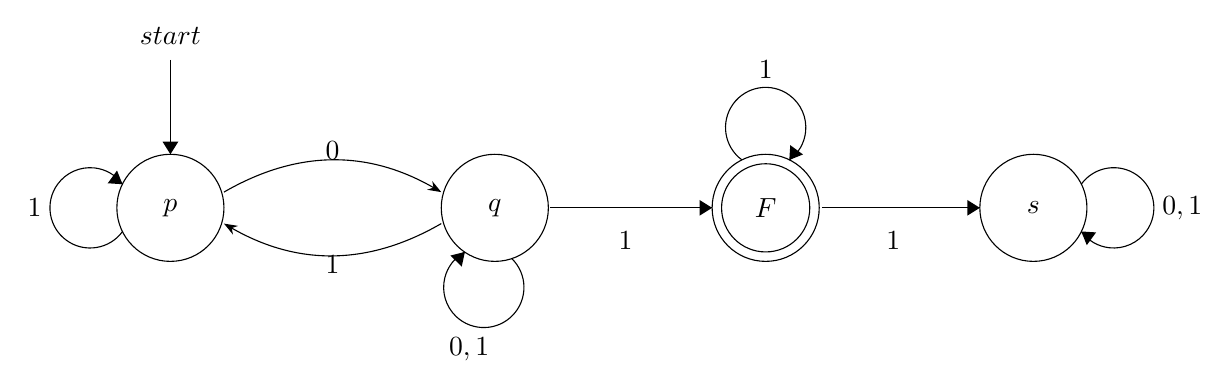
\begin{tikzpicture}[scale=0.2]
\tikzstyle{every node}+=[inner sep=0pt]
\draw [black] (9.1,-16.5) circle (3.4);
\draw (9.1,-16.5) node {$p$};
\draw [black] (29.7,-16.5) circle (3.4);
\draw (29.7,-16.5) node {$q$};
\draw [black] (46.9,-16.5) circle (3.4);
\draw (46.9,-16.5) node {$F$};
\draw [black] (46.9,-16.5) circle (2.8);
\draw [black] (63.9,-16.5) circle (3.4);
\draw (63.9,-16.5) node {$s$};
%\draw [black] (9.1,-3.6) circle (3.4);
\draw (9.1,-5.6) node {$start$};
%\draw [black] (12.8,-16.5) -- (26.3,-16.5);%p-q
\draw (12.5,-15.5) edge[bend left, above,-Stealth] node{0} (26.3,-15.5);
\draw (26.3,-17.5) edge[bend left, below,-Stealth] node{1} (12.5,-17.5); 
%\draw (18,-18) node [below] {$0$};
\draw [black] (33.2,-16.5) -- (43.5,-16.5);%q-f
\draw (38,-18) node [below] {$1$};
\fill [black] (43.5,-16.5) -- (42.7,-16) -- (42.7,-17);
\draw [black] (50.5,-16.5) -- (60.5,-16.5);%F-s
\draw (55,-18) node [below] {$1$};
\fill [black] (60.5,-16.5) -- (59.7,-16) -- (59.7,-17);
\draw [black] (9.1,-7.1) -- (9.1,-13.1);
\fill [black] (9.1,-13.1) -- (9.6,-12.3) -- (8.6,-12.3);
\draw [black] (6.063,-17.999) arc (-36:-324:2.55);
\draw (0.95,-16.5) node [left] {$1$};
\fill [black] (6.06,-15) -- (5.71,-14.13) -- (5.12,-14.94);
\draw [black] (30.768,-19.714) arc (46.11307:-241.88693:2.55);
\draw (28.07,-24.74) node [below] {$0,1$};
\fill [black] (27.8,-19.3) -- (26.88,-19.53) -- (27.6,-20.23);
\draw [black] (45.401,-13.463) arc (234:-54:2.55);
\draw (46.9,-8.35) node [above] {$1$};
\fill [black] (48.4,-13.46) -- (49.27,-13.11) -- (48.46,-12.52);
\draw [black] (66.937,-15.001) arc (144:-144:2.55);
\draw (72.05,-16.5) node [right] {$0,1$};
\fill [black] (66.94,-18) -- (67.29,-18.87) -- (67.88,-18.06);
\end{tikzpicture}
\end{center}
每一个state里面存在一个proposition,它表示这个proposition is hold at this state,自然地states就变成了possible worlds. state现在可以接受多个输入$\{0,1\}$,那么这里就表示我们有两个relations $\rho_0$和$\rho_1$,对应我们需要两个pair来构建不同的modality $(\square_0,\Diamond_0)$和$(\square_1,\Diamond_1)$,它们都是用于描述某个state的successor. 因此这里可以对应上一个Kripke structure, 对上图我们可以列举几个vaild formula.
$$
\begin{aligned}
&K \vDash \neg \Diamond_0 F && \text{does not end with 0} \\
&K \vDash p \to \Diamond_0 p &&\text{$p$ has a 1-loop} \\
&K \vDash \Diamond_0~true && \text{never stuck with input 0} \\
&K \vDash \Diamond_1~true && \text{never stuck with input 1} \\
\end{aligned}
$$
再看一个稍微复杂一点
$$
K \vDash F \to \Diamond_0(\neg \Diamond_0 F \wedge \neg \Diamond_1 F)
$$
它意思如果某个状态$\sigma$下$F$ is hold, 那么$\sigma$ accept 0 的successors $\{s_i\}$中每个$s_i$的successors都无法hold $F$,显然这是成立的. 
\end{annotation}


\begin{definition}
\rm A system $\mathcal{S}$ of proof rules and axioms of modal logic is sound iff, for all formulas $\psi$ and all sets of formulas $\Phi$:
$$
\Phi \vdash_S \psi~\text{implies}~\Phi \vDash_g \psi
$$
\end{definition}


\begin{annotation}
\rm 上述soundness实际在建立关于axiomatic modal logic和semantic modal logic之间的一座桥,这座桥需要每一个axiom make sense. 
\end{annotation}

\begin{lemma}
\rm Kripke axiom $\square(\phi \to \psi) \to (\square\phi \to \square\psi)$ is sound.
\end{lemma}

\begin{proof}
\rm 首先给定任意一个Kripke structure $K$. 我们需要证明
$$
K,s \vDash \square(\phi \to \psi) \to (\square\phi \to \square\psi).
$$
因此假设其前提
$$
\begin{aligned}
&K,s \vDash \square(\phi \to \psi) \\
&K,s \vDash \square\phi
\end{aligned}
$$
那么对应所有满足$s \rho t$的successor $t$, 都有
$$
\begin{aligned}
&K,t \vDash \phi \to \psi \\
&K,t \vDash \phi
\end{aligned}
$$
自然地这里有$K,t \vDash \psi$,于是$K,s \vDash \Diamond \psi$. 
\end{proof}

\begin{lemma}
\rm G\"{o}del Rule $\infer{\square\phi}{\phi}$ is sound.
\end{lemma}

\begin{proof}
注意这里的结论是建立在global assumption上的,即$K,s \vDash \phi$ for any $s \in W$,证明过程是显然的.
\end{proof}

\begin{lemma}
\rm A Kripke frame $(W,\rho)$ is reflexive, that $\rho$ is reflexive, if and only if $K,s \vDash \square q \to q$ for all Kripke structures $K = (W,\rho,v)$. 
\end{lemma}

\begin{proof}
($\Rightarrow$) 若$(W,\rho)$ is reflexive, 这是显然的.

($\Leftarrow$) 若$K,s \vDash \square q \to q$ for all Kripke structures $K = (W,\rho,v)$. 假设存在一个$r$ such that $(r,r) \notin \rho$, 构造一个比较巧妙地valuation $v$
$$
v(s)(q) = \left\{
\begin{aligned}
&true && \text{if}~r \rho s \\
&false && \text{otherwise}
\end{aligned}
\right.
$$
那么显然有$K,r \vDash \square q$,根据前提这里有$K,r \vDash q$,而根据valuation这里就$r$存在一个successor是它自己,即$(r,r)$与假设矛盾. 
\end{proof}

\begin{lemma}
\rm  A Kriple frame $(W,\rho)$ is transitive, that $\rho$ is transitive, if and only if $K,s \vDash \square q \to \square\square q$ for all Kripke structures $K=(W,\rho,v)$. 
\end{lemma}

\begin{proof}
\rm ($\Rightarrow$) 若$(W,\rho)$ is transitive, 给定$K,s \vDash \square q$,对于$s$的任意一个successor $t$($s \rho t$)则有$K,t \vDash p$,进一步对$t$的任意一个successor $r$($t \rho r$),考虑transitive $s \rho r$,那么有$K,r \vDash p$. 由于$t$和$r$的任意性,因此$K,s \vDash \square\square p$. 

($\Leftarrow$) 若Kriple frame满足对任意的valuation $v$都有$K,s \vDash \square q \to \square\square q$. 假设$(W,\rho)$不是transitive, 那么存在$r_1,r_2,r_3 \in W$ such that $r_1 \rho r_2, r_2 \rho r_3$ and $(r_1,r_3) \notin \rho$. 构造一个valuation $v$
$$
v(s)(q) = \left\{
\begin{aligned}
&true && \text{if}~r_0 \rho s \\
&false && \text{otherwise}
\end{aligned}
\right.
$$
那么$K,r_0 \vDash \square q$,但是因为$(r_0,r_3) \notin \rho$,因此$K, r_0 \nvDash \square\square q$,和假设前提矛盾了. 
\end{proof}

\begin{annotation}
\rm 这座需要两边的支撑一样高,给定特定axiomatic modal logic, 我们得到找到与之对应的semantic modal logic,我们的手法就是sketch it from basic Kripke frame. 当我们尝试构造了一部分之后,我们需要让其make sense,上述lemma利用formula来characterize是一个不错的选择. 
\end{annotation}

\begin{definition}
\rm (\redt{characterization})Let $C$ be a class of Kripke frames and $\phi$ a formula in modal logic.  Formula $\phi$ characterizes $C$, if for every Kripke frame $(W,\rho)$:
$$
(W,\rho) \in C ~\text{iff for each}~v: K,s \vDash \phi~\text{holds for}~K=(W,\rho,v).  
$$
\end{definition}

\begin{theorem}
\rm (\redt{soundness of $\mathcal{S}4$})The Kriple proof rules for $\mathcal{S}4$ are sound for the class of reflexive and transitive frames.
\end{theorem}

\begin{theorem}
\rm The conjunction of the following two multimodal formulas
$$
\begin{aligned}
&\square_a p \to (p \wedge \square_a\square_b p) \\
&\square_a(p \to \square_b p) \to (p \to \square_a p)
\end{aligned}
$$
characterizest the class of all multimodal kripke frames $(W, \rho_a,\rho_b)$ such that $\rho_a$ is the reflxive, transitive closure of $\rho_b$. 
\end{theorem}

\begin{proof}
\rm ($\Leftarrow$) 如果$(W, \rho_a, \rho_b)$is Kripke frame where $\rho_a$ is the reflexive, transitive closure of $\rho_b$. 对于一个formula只要注意到$\square_a\square_a p \to \square_a\square_b p$即可,可以从需要考虑的successors数量来证明. 对于第二个formula, 先给一个思考图
$$
% https://tikzcd.yichuanshen.de/#N4Igdg9gJgpgziAXAbVABwnAlgFyxMJZABgBoBGAXVJADcBDAGwFcYkQEBfU9TXfQigBMFanSat2ORGgAEAHXk4IC+XACOzegCcYAfQBGsuQD9FOGAA8cwemCicTxkN17Y8BIgHZRNBizZEEG0XHhAMdwEiABZSYjF-SSCAdz1gLE5Qt35PFABWOISJQJBU9IBqckzOMRgoAHN4IlAAM20IAFskMhBlJHI-YvY4VW0ACwhDAD0AKlkcLJA2zv6aPsQRcQCpUYnpuZDXJfauxABmNYgkWK2kkANEVKxdyaMyrErqsOXTgd6r840RhYMAlKD0OBjOogQbbIIGGaLH7XS5ITbA0HscGQ6Gwu4IpEnbqowH3GD2JBnHqJEojRTjV6zFyUThAA
\begin{tikzcd}
                                                                    &  &                                                                                            &  & w_{i} \arrow[r, "b:w_i \rho_b w_{i+1}"] & w_{i+1} \arrow[rrd, "b*", dashed] &  &   \\
s \arrow[rr, "s \rho_b^* t"] \arrow[rrrru, "s \rho_b^* w_i", bend left] &  & t:p \to \square_b p ~\text{and}~ p \arrow[rrrrr, "t \rho_b^* r"] \arrow[rru, "b*", dashed] &  &                                         &                                   &  & r
\end{tikzcd}
$$
这里$\rho_a  = \rho_b^*$. 这里证明手法是
$$
\square_a(p \to \square_b p) \to \square_a(p \to \square_a p) ~\text{and}~ \square_a(p \to \square_a p) \to (p \to \square_a p)   
$$
最重要是证明第一个implication,第二个implication是前面已经证明过的reflexive. 对于第一个implication它描述的是首先给出前提(1)$\square_a(p \to \square_b p)$即$s \rho_b^* t$. 然后我们想要将$t$中$p \to \square p$扩展至$p \to \square_b^* p$,因此再给一个假设前提$t$ holds p,我们来考察$\square_b^* p$是否成立即$t \rho_b^* r$. 这里我们需要分解$t \rho_b^* r$使其为$w_i \rho_b w_{i+1}$ for all $i < n$,其中$w_0=t$和$w_{n} = r$. 利用数学归纳法证明$K,w_i \vdash p$,这里就不详细描述了,和后面一个证明过程类似,但是说明几点: (1)$s \rho_b^* w_i$送来了$p \to \square_b p$ (2)假设前提保证了$K,w_i \vDash p$. 因此$K,w_{i+1}\vDash p$. 

($\Rightarrow$) 如果$(W, \rho_a, \rho_b)$is Kripke frame such that above formulas are vaild in it for any valution $v$. 我们得证明$\rho_a = \rho_b^*$. 这种证明两个集合相等的手法,还是用两边证.

先证\bluet{$\rho_a \subseteq \rho_b^*$}. 取任意的$(s,t) \in \rho_a$,我们得证明$(s,t) \in \rho_b^*$. 还是构造一个特殊的valuation
$$
v(w)(q) = \left\{
\begin{aligned}
&true && \text{if}~(s,w) \in \rho_b^* \\
&false && \text{otherwise}
\end{aligned}
\right.
$$
我们的思路是首先证明第二个formula的前提(1) $\square_a(p \to \square_b p)$,从而得到对应的conclusion (2) $(p \to \square_a p)$,由给定的$v$结合$\rho_b^*$的reflexive性质,自然地有$K,s \vDash p$,在使用一下(2)得到$K,t \vDash p$, 这样就有$(s,t) \in \rho_b^*$.  证明(1)思路是依然是假设前提: 给定$s \rho_a w$且$K,w \vDash p$,实际上$(s,w) \in \rho_b^*$. 考虑下面的思考过程
$$
% https://tikzcd.yichuanshen.de/#N4Igdg9gJgpgziAXAbVABwnAlgFyxMJZABgBpiBdUkANwEMAbAVxiRAQF9T1Nd9CUAJnJVajFmwDuiAARoQXHtjwEiAFhHV6zVohCSA5AtEwoAc3hFQAMwBOEALZIyIHBCQBGLeN0g6suBkAHSDbAAsIAH0AIwA9ACoZSRBqBjpomAYABV4VARAGGGscBW4QO0dnajckYTEdNkCQ8Ki4xMMUgvTMnOV+NkLizoywKCQAZmJFcvsnRC9Xd0Q67Qk9aNlJZoiYhI7U7uzc-r1Bko4KDiA
\begin{tikzcd}
s \arrow[rr, "a: s \rho_b^* w"] \arrow[rrrr, "s \rho_b^* w'", bend left] &  & w: p \arrow[rr, "b: w\rho_b^*w'"] &  & w'
\end{tikzcd}
$$
另外又给了一个$w'$满足$w \rho_b w'$,再根据$\rho_b^*$的transitive得到$s \rho_b^* w'$,从而$K,w' \vDash p$. 

再证\bluet{$\rho_a \supseteq \rho_b^*$}. 取任意的$(s,t) \in \rho_b^*$,我们要证明$(s,t) \in \rho_a$. 依然构造一个类似的valuation
$$
v(w)(q) = \left\{
\begin{aligned}
&true && \text{if}~(s,w) \in \rho_a \\
&false && \text{otherwise}
\end{aligned}
\right.
$$
我们的思路: 由于我们构造地特别的$v$有$K,s \vDash \square_a p$, 借助命题中的第一个formula得到对应的conclusion (1) $K,s \vDash p \wedge \square_a\square_b p$. 考虑下面的思考过程
$$
% https://tikzcd.yichuanshen.de/#N4Igdg9gJgpgziAXAbVABwnAlgFyxMJZABgBoBGAXVJADcBDAGwFcYkQ5E0QBfU9TLnyEUAJlLFqdJq3YB3APpYuvfiAzY8BIgFYKUhizaIQOFXwGbhRAMwSDM4yEXAsAanI9zUmFADm8ESgAGYAThAAtkhkphBI4tJG7HAABAA6aaEAFhAKAEYAegBUKTiqIeFRiDE4cYjkNIxYYE5Q9HBZviA0eTBgUEg2xBYgYZFIDbGDPX0D1TSGsiZ5iCmKWOmZOflrCq4ePOWjldNTiAlNLextHV0z-YPDlDxAA
\begin{tikzcd}
                                                                 &  & w_i:p \arrow[r, "b: w_i \rho_b w_{i+1}"] & w_{i+1}:p \arrow[rrd, dashed, bend left] &  &     \\
s:p \arrow[rrrrr, "s \rho_b^* t"] \arrow[rru, dashed, bend left] &  &                                          &                                          &  & t:p
\end{tikzcd}
$$
我们考虑将$s \rho_b^* t$拆开,设$w_i \rho_b w_{i+1}$ for all $i < n$,其中$w_0 = s$和$w_n = t$,这是可以做到的,考虑closure的构造过程. 再用一下数学归纳法证明$K, w_i \vDash p$,在$i=0$显然是成立的,假设$w_i$成立,那么根据$v$即有$s \rho_a w_i$,再利用一下(1)可以得到$K,w_i \vDash \square_b p$,因此$K,w_{i+1} \vDash p$. 最终$K,t \vDash p$,那么$(s,t) \in \rho_a$. 
\end{proof}

\begin{annotation}
\rm \bluet{回顾上面的证明手法},我们如果想要刻画两个possible worlds是否存在某种关系,例如$(r,t) \stackrel{?}{\in} \rho$,我们可以额外借助一个formula $p$和valuation $v$,仅使得所有$w$满足$r \rho w$都hold $p$. 这样如果我们能利用额外和$p$相关的条件间接证明$t$ holds $p$, 那么就可以证明$s \to t$. 我们应该意识到relations是Kripke frame固有的性质,与valuation无关因此这里我们可以任意的定义它.  
\end{annotation}

\newpage
\section{Natural Deduction}

\begin{remark}
\rm \redt{Natural deduction is a kind of proof calculus in which logical reasoning is expressed by inference rules closely related to the "natural" way of reasoning}. 
\end{remark}

\subsection{Judgments and Propositions}

\begin{definition}
\rm A \emph{judgment} is somthing we may know, this is, an object of knowledge. A judgment is \emph{evident} if we in fact know it.
\end{definition}

\begin{annotation}
\rm "A is false" (see classical logic), "A is true at time t" (see temporal logic), "A is necessarily true" or "A is possibly true" (see modal logic), "the program M has type τ" (see programming languages and type theory), "A is achievable from the available resources" (see linear logic). 
\end{annotation}

%inference rule 写一遍没意思

\subsection{Introduction and Elimination}

\begin{definition}
\rm Inference rules that introduce a logical connective is the conclusion are known as \emph{introduction rules}. i.e., to conclude "$A~\text{and}~B~true$" for propositions $A$ and $B$, one requires evidence for "$A~true$" and $B~true$. As an inference rule:
$$
\infer[\wedge I]{A \wedge B ~true}{A~true & B~true}
$$
Here $\wedge I$ stands for "conjunction introduction".
\end{definition}

\begin{annotation}
\rm 实际上面的inference rule的general form应该是
$$
\infer[\wedge I]{A \wedge B ~true}{A~prog & B~prog & A~true & B~true}
$$
这里才能帮助后面的$\vDash$ make sense. 
\end{annotation}

\begin{definition}
\rm Inference rules that describe how to deconstruct information about a compound proposition into information about its consitiuents are elimination rules. i.e., from $A \wedge B~true$, we can conclude $A~true$ and $B~true$:
$$
\infer[\wedge E_L]{A~true}{A \wedge B ~true}~~~~~~\infer[\wedge E_R]{B~true}{A \wedge B ~true} 
$$
\end{definition}

\begin{annotation}
\rm The meaning of conjunction is determinded by its \emph{verifications}.  
\end{annotation}

\subsection{Hypothetical Derivations}

\begin{definition}
\rm A \emph{hypothetical judgment} is $J_1, \cdots, J_n \vdash J$, where judgments $J_1,\cdots,J_n$ are unproved assumptions, and the judgment $J$ is the conclusion. A \emph{hypothetical deduction}(derivation) for $J_1, \cdots, J_n \vdash J$ has the form 
$$
\deduce[\vdots]{\raisebox{-1.0em}{$J$}}{J_1 & \cdots & J_n}
$$
which means $J$ is derivable from $J_1, \cdots, J_n$. 
\end{definition}

\begin{annotation}
\rm 上面的$J_1,\cdots,J_2$都可以替换成关于$J_i$的一个hypothetical derivation. 
\end{annotation}


\begin{definition}
\rm In the natural deduction calculus, an assumption is discharged when the conclusion of an inference does not depend on it, although one of the premises of the inference does\cite{tln}.
\end{definition}

\begin{annotation}
\rm Once the appropriate rules have been completed, these are known as discharged assumptions, and are not included in the pool of assumptions on which the conclusion of the rule depends\cite{discharged-proofwiki}.
\end{annotation}

\begin{annotation}
\rm hypothetical derivation要求最后的conclusion依赖的poof of assumptions不是空的. 
\end{annotation}

\begin{theorem}
\rm \redt{Deduction theorem} \[T, P \vdash Q \iff T \vdash P \to Q\].
\end{theorem}

\begin{annotation}
\rm 在deduction theorem中我们注意到第一个hypothetical judgment里面的antecedent $Q$被去掉了,在第二个hypothetical judgment的succedent里面作为一个implication的antecedent出现了,这里我们就可以说assumption $Q$ is discharged,即现在的conclusion已经不依赖它了. 那么我们是如何构造deduction theorem里面的implication的呢? 下面接着看
\end{annotation}

\begin{definition}
\rm (\redt{implication}) If $B$ is true under the assumption that $A$ is true, formly written $A \supset B$. The corresponed introduction and elimination rule as follow \[\infer[\supset\!\!I^u]{A \supset B~true}{\deduce[\vdots]{B~true}{\infer[u]{A~true}{}}}~~~~~ \infer[\supset\!\!E]{B~true}{A\supset B~true & A~true}\]
\end{definition}

\begin{annotation}
\rm \redt{Why indexed $u$} In the introduction rule, the antecedent named $u$ is discharged in the conclusion. This is a mechanism for delimiting the scope of the hypothesis: its sole reason for existence is to establish "$B~true$"; it cannot be used for any other purpose, and in particular, it cannot be used below the introduction.

上面这段话出自natural deduction的wiki,这个$u$scope了assumption $A~true$的开端,因为$A\supset B$并不依赖$A~true$, 它描述只是if $A~true$ then $B~true$. 
同时最后的introduction rule会将这个assumption $A~true$ discharged掉,表示scope在这里已经结束了. 而implication rule会将上述derivation直接总结得到一个结论,即
$$
A \vdash B \Rightarrow \cdot\vdash A \to B. 
$$
\end{annotation}

\begin{example}
\rm Considering the following proof of $A \supset (B \supset (A \wedge B))$
$$
\infer[I^u]{A \supset (B \supset (A \wedge B))~true}{\infer[I^w]{B \supset (A \wedge B)~true}{\infer[\wedge I]{A \wedge B~true}{\infer[u]{A~true}{} & \infer[w]{B~true}{}}}}.
$$

这整个derivation不是hypothetical的,因为两个assumptions $A~true$和$B~true$都已经被discharged,因此它实际上一个complete proof! 
\end{example}

\begin{definition}
\rm (\redt{disjunction}) The elimination rule for disjunction:
$$
\infer[\vee E^{u,w}]{C~true}{A \vee B ~true & \deduce[\vdots]{C~true}{\infer[u]{A~true}{}} & \deduce[\vdots]{C~true}{\infer[w]{B~true}{}}}
$$
both assumption $u,w$ are discharged at the disjunction elimination rule. 
\end{definition}


\begin{definition}
\rm The falsehood elimination rule:
$$
\infer[\perp\!\!E]{C~true}{\perp~true}
$$
\end{definition}

\begin{annotation}
\rm falsehood elimination的意义在哪? 首先你应该主要到一个特殊等价命题$A \vee \perp = A$,从$\vee$的introduction rule来看这意味$\perp~true \vdash A~true$,由于$A$是任意的,因此我们得到了$\perp~true \vdash C~true$. 
\end{annotation}

\newpage
\subsection{Harmony}

\begin{definition}
\rm \redt{Local soundness} shows that the elimination rules are not strong: no matter how we apply eliminations rules to the result of an introduction we cannot gain any new information.
\end{definition}

\begin{definition}
\rm \redt{Local completeness} shows that the elimination rules are not weak: there is always a way to apply elimination rules so that we can reconstitute a proof of the original proposition from the the results by apply intruduction ruls. 
\end{definition}

\begin{annotation}
\rm local soundness告诉你通过elimination压缩得到的东西不会比你已经知道的东西强(not strong),而local completeness告诉你合并通过elimination压缩得到的东西会得到全部你知道的信息. 
\end{annotation}


\begin{definition}
\rm Given two deduction of same judgment, we use the notion
$$
\deduce{A~true}{\mathcal{D}} \Longrightarrow_{R} \deduce{A~true}{\mathcal{D'}} 
$$
for the \redt{local reduction} of a deduction $\mathcal{D}$ to another deduction $D'$ of same judgement $A~true$. Simliarly, we have \redt{local expansion}
$$
\deduce{A~true}{\mathcal{D}'} \Longrightarrow_{E} \deduce{A~true}{\mathcal{D}}
$$
\end{definition}


\begin{definition}
\rm (\redt{substitution Principle}) If 
$$
\deduce[\mathcal{E}]{C~true}{\infer[u]{A~true}{}}
$$
is a hypothetical proof of $\mathcal{C}~true$ under the undischarged hypothesis $A~true$ labelled $u$, and 
$$
\deduce{A~true}{\mathcal{D}}
$$
is a proof of $A~true$ then
$$
\deduce[\mathcal{E}]{C~true}{\infer[u]{A~true}{\mathcal{D}}}
$$
is our notation for substituting $\mathcal{D}$ for all uses of the hypothesis labelled $u$ in $\mathcal{E}$. This deduction, also sometime written as $[\mathcal{D}/u]\mathcal{E}$ no longer depends on $u$.  
\end{definition}


\begin{example}
\rm If given a elimination rule of disjunction as follow
$$
\infer[\vee\!E_L]{A~true}{A \vee B~true}
$$
The rule a little bit stronger, since we would not be able to reduce
$$
\infer[\vee\!E_L]{A~true}{\infer[\vee\!I_R]{A \vee B~true}{B~true}}
$$
As u can see it's not local soundness. 
\end{example}


%\begin{definition}
%\rm The \redt{soundness} of proof system will assure that we can %only construct proofs of vaild arguments. That is, we want to %prove that every sentence in a proof is entailed by previous %sentenses. 
%\end{definition}

%Godel
%\begin{definition}
%\rm A deduction system is said to be complete if every %universally valid formula in the language $L$ has a proof under %the proof system.
%\end{definition}




\newpage
\subsection{Verifications and Uses}

\begin{definition}
\rm a verification should be a proof that only analyzes the consitituents of a proposition.
\end{definition}


\begin{annotation}
\rm \cite{15-317-vu} 在natural deduction中由于local reduction的存在,可能会让一个证明过程变得非常的冗余,例如在证明conjunction commutativity
$$
\infer[\supset I^u]{(A \wedge B) \supset (B \wedge A)~true}{\infer[\wedge I]{B \wedge A~true}{\infer[\wedge E_2]{B~true}{\infer[\wedge I]{A \wedge B~true}{\infer[\wedge E_1]{A~true}{\infer[u]{A \wedge B ~true}{}}  &  \infer[\wedge E_2]{B~true}{\infer[u]{A \wedge B ~true}{}}}}  &  \infer[\wedge E_1]{A~true}{\infer[u]{A \wedge B ~true}{}}}}
$$
其中左上角的local reduction显然是冗余的. 这样对于谈论某个具体proposition的proof时就会出现问题,因为the shape of proof is not decidable. 同时我们也希望未来能够设计出一个tool用于deviates proofs automatically,也就是search proof automatically. 因此从natural deduction上诞生了一个新的calculus,它会在syntax level上来施加一些限制,借此限制the shape of proof. 最后我们将证明这个calculus引入的restrictions不会产生side-effect.   
\end{annotation}


\begin{definition}
\rm Writing $A\uparrow$ for the judgment "A has a verification". Naturally, this should mean that $A$ is true,  and that the evidence for that has a special form.
\end{definition}

\begin{definition}
\rm Writing $A\downarrow$ for the judgment "A may be used". $A\downarrow$ should be the case when either $A~true$ is a hypothesis, or $A$ is deduced from a hypothesis via elimination rules. 
\end{definition}

\begin{annotation}
\rm 我觉得下述两种理解方式更为明确易懂
\begin{itemize}
	\item $A \uparrow$ denotes that we are searching for a verfication of $A$;
	\item $A  \downarrow$ denotes that we are allowed to use $A$. 
\end{itemize}
\end{annotation}

\begin{annotation}
\rm 上述两个definitions里面隐藏着非常重要但有点不正式的结论:If $A$ has a vertification then $A$ true, 反之依然. 后面我们将形式化地证明它们. 
\end{annotation}

\begin{definition}
\rm For conjunction. 
$$
\begin{aligned}
&\infer[\wedge I]{A \wedge B\uparrow}{A \uparrow & B \uparrow} &&& \infer[\wedge E_L]{A \downarrow}{A \wedge B \downarrow} &&&& \infer[\wedge E_R]{B \downarrow}{A \wedge B \downarrow}
\end{aligned}
$$
\end{definition}


\begin{definition}
\rm For implication
$$
\begin{aligned}
&\infer[\supset^u]{A \supset B \uparrow}{\deduce[\vdots]{B\uparrow}{\infer[u]{A\downarrow}{}}} &&& \infer[\supset E]{B \downarrow}{A \supset B \downarrow & A \uparrow}
\end{aligned}
$$
\end{definition}

\begin{annotation}
\rm (\redt{why implication}) In order to have a verification of $A \supset B$, we need a proof of $B$ and we are given an assumption $A$ to work with. Therefore, we will need a verification of $B$ and we are allowed to use $A$. 

When using an implication statement in a proof, we need to show that the antecedent holds, so we need a verification of it. Only then we are allowed to use the consequent.
\end{annotation}

\begin{example}\label{use-is-weaker}
\rm
$$
\infer{((A \supset A) \supset B) \supset B \uparrow}{\infer{B ~?}{(A\supset A) \supset B ~? & \infer{A \supset A ~?}{\infer{A~?}{A~?}}}}
$$
\end{example}

\begin{example}\label{early-verification-and-truth}
\rm 
$$
\infer[\supset I^u]{(A \wedge B) \supset A~true}{\infer[\wedge E_L]{A~true}{\infer[u]{A\wedge B~true}{}}}
$$
那么它对应上verification和use
$$
\infer[\supset I^u]{(A \wedge B) \supset A~?}{\infer[\wedge E_L]{A \downarrow}{A \wedge B \downarrow}}
$$
一切都非常奇怪,这个verification和use到底是怎样对应truth? 从前面两个例子都可以清晰地感觉到一个阻力,即
$$
\deduce[???]{A \uparrow}{A \downarrow}
$$
就是当我们在use $A$的时候,实际上存在一个$A$ has a verification. 
\end{example}


\begin{definition}
\rm For disjunction
$$
\begin{aligned}
&\infer[\vee I_L]{A \vee B \uparrow}{A \uparrow} &&& \infer[\vee I_R]{A \vee B \uparrow}{B \uparrow} &&&  \infer[\vee E^{u,w}]{C \uparrow}{A \vee B \downarrow & \deduce[\vdots]{C\uparrow}{\infer[u]{A\uparrow}{}} & \deduce[\vdots]{C\uparrow}{\infer[w]{B\downarrow}{}}}
\end{aligned}
$$
\end{definition}


\begin{definition}
\rm For truth and falsehood.
$$
\begin{aligned}
& \infer[\top I]{\top \uparrow}{} &&& \infer[\perp E]{C\uparrow}{\perp \downarrow}
\end{aligned}
$$
\end{definition}

\begin{annotation}
\rm $\perp \downarrow$ signifies a contradiction from our hypotheses.
\end{annotation}

\begin{annotation}
\rm the elimination rule of disjunction and falsehood里面出现conclusion $C \uparrow$也很奇怪,为什么不是$C \downarrow$?
\end{annotation}

\begin{definition}\label{arrow switch of atomic}
\rm For atomic propositions.
$$
\infer[\downarrow\uparrow]{P \uparrow}{P \downarrow}.
$$
\end{definition}

\begin{annotation}
\rm 当引入上述的arrow switch之后我们可以回答前面的种种问题了. 首先是example \ref{use-is-weaker},假设其中的$A,B$都是atomic proposition,则
$$
\infer[\supset I^w]{((A \supset A) \supset B) \supset B \uparrow}{\infer[\downarrow\uparrow]{B \uparrow}{\infer{B ~\downarrow}{\infer[w]{(A\supset A) \supset B ~\downarrow}{} & \infer[\supset I^u]{A \supset A ~\uparrow}{\infer[\downarrow\uparrow]{A~\uparrow}{\infer[u]{A~\downarrow}{}}}}}}
$$
同时如果将implication emilination的premise换成$A \downarrow$,在找$A \supset A \downarrow$的proof时就被卡住了. example \ref{early-verification-and-truth}类似. 那么有一个很自然的问题这个arrow switch能不能推广到任意的propositions上呢? 本质上是没有问题的,例如
$$
\infer[\supset I^u]{A \supset A \uparrow}{\infer[\downarrow\uparrow]{A \uparrow}{\infer{A \downarrow}{A \supset A \downarrow & \infer[\downarrow\uparrow]{A \uparrow}{\infer[u]{A~\downarrow}{}}}}}
$$
但是这样的语法又会使得proof search space变大,并不符合我们的初衷,因此我们只将arrow switch放在的了atomic proposition上,这样做的后果你也可以看到,需要将connectives都展开.  

再来思考另外一种arrow switch
$$
\infer[\uparrow\downarrow]{F \uparrow}{&F \downarrow&}
$$
这个人在本质上也是没有问题的,当我们有一个关于$F$的verification,我们当然可以use it. 但是引入它同样会造成我们的proof search space,就像classical logic中的tautologies,我们可以在任何proof中使用它,但是有时候是没有意义的. 同在emilinotation rule of disjunction and falsehood中的conclusion中我们都是使用的verification,而不是use,也是为了防止后续使得我们的proof变得复杂. 
\end{annotation}

\begin{theorem}
\rm (\redt{Global Soundness}) $\deduce[\vdots]{\text{If}~A \uparrow~\text{and}~C\uparrow~\text{then}~C \uparrow}{A \downarrow}$
\end{theorem}

\begin{annotation}
\rm Global Soundness意味着如果if the verification formula of $C$ under the verification formula $A$,那么在$C$中使用$A$,并不会得到任何其他new informations.
\end{annotation}

\begin{theorem}
\rm (\redt{Global Completeness}) If $A \downarrow$, then $A \uparrow$. 
\end{theorem}

\begin{annotation}
\rm Global completeness意味着如果我们确定formula $A$在某种情况下可以使用,那么在相同的assumptions下我们可以推导出一个关于它的verification. 这在前面关于$\downarrow\uparrow$转换规则的annotation中已经见识过一个特殊例子了. 
\end{annotation}

\newpage
\subsection{Notational Definition}

\begin{definition}
\rm A \redt{notational definition} gives the meaning of the general form of a proposition in terms of another proposition whose meaning has already been defined.
\end{definition}

\begin{example}
\rm We can define logical equivalence, written $A \equiv B$ as 
$$
(A \supset B) \wedge (B \supset A).
$$ 
\end{example}

\begin{example}
\rm We can define negation $\neg A$ as 
$$
\neg A = (A \supset \perp) \Longrightarrow \infer[\neg I]{\neg A}{\deduce[\vdots]{\perp}{A}}
$$
We also can give the introduction rule of falsehood.
$$
\infer[\perp I]{\perp}{\neg A & A}
$$
so $\perp$ actually means any contradictions. moreover double negation is coming.
\end{example}

\begin{annotation}
\rm notaional definition可以看做用已有的东西构造出一些东西. 与之对应的是我们可以直接符号化的给出某个新的定义,称之为symbolic definition. 
\end{annotation}

\newpage
\subsection{Soundness and Completeness of Native Natural Deduction}

\begin{definition}
\rm \cite{cs245-nd}\redt{Soundness} of natural deduction means that the conclusion of proof is always a logical consequence of the premises. That is
$$
\text{If}~\Sigma \vdash \alpha, \text{then}~\Sigma \vDash \alpha. 
$$ 
\end{definition}


\begin{definition}
\rm \redt{Completeness} of natural deduction means that all logical consequences in propositional logic are provable in natural deduction. That is,
$$
\text{If}~\Sigma \vDash \alpha, \text{then}~\Sigma \vdash \alpha.
$$ 
\end{definition}

\begin{annotation}
\rm 其中$\Sigma \vdash \alpha$, 表示存在一个以$\Sigma$作为premise得到conclusion为$\alpha$的proof. 而$\Sigma \vDash \alpha$,就考虑两端的proposition加上truth-falsehood了, 即如$\Sigma^t = True$则有$\alpha^t = True$.

对于soundness的证明,我们需要根据$\alpha$的结构来做归纳,而后再考虑赋予其true/false来考虑. 这里记录一下对于结构归纳它是怎样对应一般归纳法命题$P(n)$结构上,这里的$n$应该对应$\alpha$的bottom-up derivation里面的maximum depth of line. 

而对于completeness的证明,相对来说会复杂一点. 我们需要下面3个lemma. 有一个疑问不引入negation是不是还说明不了completeness?
\end{annotation}

\begin{lemma}
\rm If $\Sigma =\{\alpha_0,\alpha_1,\cdots,\cdots,\alpha_n\} $ and $\Sigma \vDash \beta$, then
$$
\emptyset \vDash (\alpha_0 \to (\alpha_1 \to (\cdots \to (\alpha_n \to \beta)\cdots)).
$$
\end{lemma}

\begin{annotation}
\rm Deduction theorem体现的淋漓尽致,将$\beta$完美转换成了一个tautology. 
\end{annotation}

\begin{lemma}\label{how-to-construct-provable-formula}
\rm For any well-form formula $\gamma$ containing atoms $p_1,p_2,\cdots,p_n$ and any valuation $t$, we have 
\begin{enumerate}
	\item If $\gamma^t = True$ then $\widehat{p}_1,\widehat{p}_2,\cdots,\widehat{p}_n \vdash \gamma$;
	\item If $\gamma^t = False$ then $\widehat{p}_1,\widehat{p}_2,\cdots,\widehat{p}_n \vdash \neg\gamma$;
\end{enumerate}
where defines $\widehat{p}_i$ as follow
$$
\widehat{p}_i = \left\{
\begin{aligned}
&p_i && \text{if}~p_i^t = True \\
&\neg p_i && \text{if}~p_i^t = False
\end{aligned}
\right.
$$
\end{lemma}

\begin{example}
\rm 若$\gamma = p \to q$,我们可以构造一个真值表
\begin{center}
\begin{tabular}{|c|c|c|c|}
\hline
$p$ & $q$ & $p \to q$ & Claim \\ 
$T$ & $T$ & $T$ & $p , q \vdash p \to q$ \\
$T$ & $F$ & $F$ & $p , \neg q \vdash \neg(p \to q)$ \\
$F$ & $T$ & $T$ & $\neg p , q \vdash p \to q$ \\
$F$ & $F$ & $T$ & $\neg p , \neg q \vdash p \to q$ \\ 
\hline
\end{tabular}
\end{center}
那么上面的claims是怎么来的呢?我们可以来分别证明, 对于第一行
$$
\infer[u]{p \to q~true}{\infer{q~true}{\infer[u]{p~true}{} & q~true}}
$$
感觉有点奇怪,这里需要用到vars inference rule, 这里相对于对$q \vdash p \to q$的weaken premise. 对于第二行
$$
\infer[u]{\neg (p \to q)~true}{\infer{\perp}{\infer{q}{\infer[u]{p \to q~true}{} & p~true} & \neg q ~true}}
$$
对于第三行
$$
\infer[u]{p \to q~true}{\infer{q~true}{\infer{\perp}{\infer[u]{p~true}{} & \neg p ~true}}}
$$
对于第四行,和第三行类似. 可以看的出来这个lemma非常深刻,\bluet{只要将atoms调整为在当前valuation下都是true的命题,结论再对应调整,就可以构造一个对应的proof}. 
\end{example}

\begin{lemma}\label{tautologies-are-provable}
\rm For any well-formed formula $\gamma$, if $\emptyset \vDash \gamma$, then $\emptyset \vdash \gamma$. 
\end{lemma}

\begin{annotation}
\rm Lemma \ref{tautologies-are-provable}一句话概况就是tautologies are provable. 其证明过程可以用Lemma \ref{how-to-construct-provable-formula}来说明. 现在$\gamma$是一个tautology,那么对于所有的valuation都有$\gamma^t = true$,这有什么用呢? 这里还需要引入另外一种tautology $p \vee \neg p$,配合emilination rule of $vee$,即
$$
\infer{\gamma}{(p_1 \vee \neg p_1) & (p_2 \vee \neg p_2) & \cdots & (p_n \vee \neg p_n)&\deduce[\vdots]{\gamma}{\infer{}{\infer{p_1}{} & \cdots & \infer{p_n}{}}} & \cdots & \deduce[\vdots]{\gamma}{\infer{}{\infer{\neg p_1}{} & \cdots & \infer{\neg p_n}{}}}}
$$
这里需要考虑有$2^n$个cases,每一个对应一种valuation,又因为$\gamma$是tautology,因此最后的conclusion也都是$\gamma$. 
\end{annotation}

\begin{lemma}
\rm If $\emptyset \vdash (\alpha_0 \to (\alpha_1 \to (\cdots \to (\alpha_n \to \beta)\cdots))$, then $\{\alpha_0, \alpha_1,\cdots,\alpha_n\} \vdash \beta$, that is, $\Sigma \vdash \beta$. 
\end{lemma}

\newpage
\subsection{Derived Rules of Inference}

\begin{example}
\rm 
$$
\infer{A \supset C~true}{A \supset B~true & B \supset C~true}
$$
is a derived rule of inference. Its derivation is the following:
$$
\infer[\supset I^u]{A \supset C~true}{\infer[\supset E]{C~true}{B \supset C~true & \infer[\supset E]{B~true}{A \supset B~true & \infer[u]{A~true}{}}}}
$$
\end{example}

\begin{annotation}
\rm 关于derivation的推导这里有一些strategies在里面
\begin{itemize}
	\item 使用introduction rule从下至上,即我们想要什么;
	\item 使用elimination rule从上至下,即我们知道什么.
\end{itemize}
\end{annotation}

\begin{example}
\rm Modus tollens(这玩意不就是逆否命题)
$$
\infer[MT]{\neg A}{A \to B & \neg B}.
$$
\end{example}


\newpage
\subsection{Curry-Howard Conrrespondence}

\begin{definition}
\rm Curry-Howard correspondence is between the natural deduction and simply-typed $\lambda$-calculus at three levels
\begin{itemize}
	\item propositions are types;
	\item proofs are programs; and
	\item simplification of proofs is evaluation of programs.
\end{itemize}
That is
\begin{center}
\begin{tabular}{c|c}
Types & Propositions \\
\hline
Unit types (1) & Truth ($\top$)\\
\hline
Product type ($\times$) & Conjunction ($\wedge$) \\
\hline
Union type ($+$)& Disjunction ($\vee$) \\
\hline
Function type ($\to$) & Implication ($\supset$)\\
\hline
Void types (0) & False ($\perp$)
\end{tabular}
\end{center}
Every typing rule has a correspondence with a deduction rule. 
\end{definition}


\begin{example}
\rm The typing derivation of the term $\lam{a}{\lam{b}{\left<a,b\right>}}$ can be seen as a deduction tree proving $A \supset B \supset A \wedge B$.
\[
\begin{aligned}
	\infer[abs]{\Gamma\vdash\lam{x:A}{\lam{y:B}{\left<x,y\right>}}:A \to B \to A \times B}{\infer[abs]{\Gamma\vdash \lam{y:B}{\left<a,y\right>}:B \to A \times B}{\infer[pair]{\Gamma\vdash \left<a,b\right>: A \times B}{\infer[var]{\Gamma\vdash a:A}{a:A \in \Gamma} & \infer[var]{\Gamma\vdash b:B}{b:B \in \Gamma}}}} & \iff & 
	\infer[\supset I^u]{A \supset B \supset A \wedge B~true}{\infer[\supset I^w]{B \supset A \wedge B~true}{\infer[\wedge \wedge I]{A \wedge B ~true}{\infer[u]{A~true}{} & \infer[w]{B~true}{}}}}		
\end{aligned}
\]
\end{example}

\begin{annotation}
\rm 从上面例子中看的出来,the inference rule of natural deduction缺点什么,我也可以给原本每个inference rule都加上the annotation for proof terms. \cite{FP-pap}那么这里$M:A$有两种解释:
\begin{enumerate}
	\item $M$ is proof term for proposition $A$;
	\item $M$ is a program of type $A$. 
\end{enumerate}
这样解释Curry-Howard ismorphism或许方便一点. 让proof terms make sense: 我们有"if $M:A$ then $A~true$",反过来"if $A~true$ then $M:A$". 例如我们可以将the proof term of $A \wedge B~true$看做一个pair包含两个subterm,一个关于$A~true$和另一个关于$B~true$.
$$
\infer[\wedge I]{\left<M,N\right>: A \wedge B}{M:A & N:B}
$$
那么the elimination rule of conjunction对应一个natural projection.
$$
\begin{aligned}
\infer[\wedge E_L]{\pi_1 M:A}{M:A \wedge B} &&& \infer[\wedge E_R]{\pi_2 M:B}{M:A \wedge B} 
\end{aligned}
$$ 
\end{annotation}


\begin{example}
\rm 通过Curry-Howard isomorphism我们可以将我们想要证明的judgment转换到type system中,你会看到非常的便利! 例如
$$
(A \supset (B \wedge C)) \supset (A \supset B) \wedge (A \supset C)~true
$$
等价于
$$
\lam{x}{\left<\lam{y}{\pi_1(x~y)},\lam{y}{\pi_2(x~y)} \right>}: (A \to B \times C) \to (A \to B) \times (A \to C)
$$
一个implication被转换成了对应的abstraction,此时我们肯定会想如果给一个false proposition是不是就转不了? 例如
$$
(A \supset B) \supset (B \supset A)
$$
显然我们无法在现有type system构造出一个合理的abstraction使得$(A \to B) \to (B \to A)$.

迎面走来的问题是: 给定一个proposition true, 是否有其他的term with type和它对应呢? 显然是有的,
$$
\lam{z}{\lam{x}{\left<\lam{y}{\pi_1(x~y)},\lam{y}{\pi_2(x~y)} \right>}}z'
$$
那这是不是违反Curry-Howard isomorphsim了呢? 其实并不是,这里的对应是指proof terms和deduction of proposition true,  显然deduction变了,对应的proof terms也要变. 
\end{example}


\newpage
\section{More Delicate}

\subsection{Natural Deduction in Sequent Nation}

\begin{definition}
\rm A sequent is a pariticular form of hypothetical judgement
$$
A_1, \cdots, A_n \vdash C.
$$
where $A_1,\cdots,A_n$ and $C$ are well-defined formulas.
\end{definition}

\begin{definition}
\rm The correspondence between natural deduction and natural deduction in sequent nation.
\begin{center}
\begin{tabular}{|c|c|}
\hline$\infer[\wedge I]{A \wedge B~true}{A~true & B~true}$ & $\infer[\wedge I]{\Gamma \vdash A \wedge B}{\Gamma \vdash A & \Gamma \vdash B}$ \rule{0mm}{10mm} \\
\hline$\infer[\wedge E_1]{A~true}{A \wedge B~true}$ \quad $\infer[\wedge E_2]{B~true}{A \wedge B~true}$ & $\infer[\wedge E_1]{\Gamma \vdash A}{\Gamma \vdash A \wedge B}$ \quad $\infer[\wedge E_2]{\Gamma \vdash B}{\Gamma \vdash A \wedge B}$ \rule{0mm}{10mm} \\
\hline$\infer[\vee I_1]{A \vee B~true}{A~true}$ \quad $\infer[\vee I_2]{A \vee B~true}{B~true}$ & $\infer[\vee I_1]{\Gamma \vdash A \vee B}{\Gamma \vdash A}$ \quad $\infer[\vee I_2]{\Gamma \vdash A \vee B}{\Gamma \vdash B}$ \rule{0mm}{10mm} \\
\hline $\infer[\vee E^{u,w}]{C~true}{A \vee B ~true & \deduce[\vdots]{C~true}{\infer[u]{A~true}{}} & \deduce[\vdots]{C~true}{\infer[w]{B~true}{}}}$ & $\infer[\vee E]{\Gamma \vdash C}{\Gamma \vdash A \vee B & \Gamma, A \vdash C & \Gamma, B \vdash C}$ \rule{0mm}{18mm} \\
\hline $\infer[\supset\!\!I^u]{A \supset B~true}{\deduce[\vdots]{B~true}{\infer[u]{A~true}{}}}$ & $\infer[\supset\!\!I]{\Gamma \vdash A \supset B}{\Gamma,A \vdash B}$ \rule{0mm}{18mm}  \\
\hline $\infer[\supset\!\!E]{B~true}{A\supset B~true & A~true}$ & $\infer[\supset\!\!E]{\Gamma \vdash B}{\Gamma \vdash A\supset B & \Gamma \vdash A}$ \rule{0mm}{10mm} \\
\hline $\infer[\top I]{\top ~true}{}$ & $\infer[\top I]{\Gamma \vdash \top}{}$ \rule{0mm}{10mm} \\
\hline $\infer[\perp E]{C~true}{\perp~true}$ & $\infer[\perp E]{\Gamma \vdash C}{\Gamma \vdash \perp}$ \rule{0mm}{10mm}\\
\hline Hypothesis discharging & $\infer[hyp]{\Gamma,A \vdash A}{}$ \rule{0mm}{10mm}\\
\hline Substitution & $\infer[subst]{\Gamma \vdash C}{\Gamma, A \vdash C & \Gamma \vdash A}$ \rule{0mm}{10mm}\\
\hline
\end{tabular}
\end{center}
\end{definition}

\begin{annotation}
\rm (\redt{detail of correspondence}) 其中$\Gamma$是一个set of formulas,它可以是empty set. 思考上述sequent形式下的natural deduction,我们应该用bottom-up的视角来观察. 试想我们在没有additional assumptions证明一个formulas,在最开始$\Gamma$应该是empty的,随着我们不断apply上述规则过程中将不断的填充$\Gamma$. 那么什么时候证明算接结束了呢? 在natural deduction中我们从下往上使用introduction rules,并添加相应的assumptions,再从上往下使用emilination rules,直到它们在中途相遇,这时候我们的证明就结束了,当证明结束的时候,此时所有的assumptions都应该被discharge了,这个操作对应到sequent形式下就是上述hyp rule,在利用sequent构造proof的时候,总是以hyp rule结束的.

显然sequent提供了一种收集assumptions的方式,使得assumptions和需要证明的formula总是在一个level,一旦某个assumption建立之后,以此往后的证明过程中这个assumption都是visible的.    
\end{annotation}

\begin{example}
\rm A proof in sequent form.
$$
\infer[\supset I]{\vdash (A \supset B) \supset ((A\wedge C) \supset (B \wedge C) ) }{\infer[\supset I]{A \supset B \vdash (A\wedge C) \supset (B \wedge C)}{\infer[\wedge I]{A \supset B,(A\wedge C) \vdash  (B \wedge C)}{\infer[\supset\!\!E]{A \supset B,(A\wedge C) \vdash B}{\infer[hyp]{A \supset B,(A\wedge C) \vdash A \supset B}{} & \infer[\wedge E_1]{A \supset B,(A\wedge C) \vdash A}{\infer[hyp]{A \supset B,(A\wedge C) \vdash A \wedge C}{}} } & \infer[\wedge E_2]{A \supset B,(A\wedge C) \vdash C}{\infer[hyp]{A \supset B,(A\wedge C) \vdash A \wedge C}{}}}}}
$$
\end{example}

\begin{definition}
\rm We say a rule is \redt{admissible} if all proofs using the rule can be transformed into proofs that do not use the rule.
\end{definition}

\begin{lemma}
\rm The \emph{subst} rule is admissible.
\end{lemma}

\begin{proof}
我们可以将其替换为等价的形式
$$
\infer[subst]{\Gamma \vdash C}{\Gamma, A \vdash C & \Gamma \vdash A} ~~\leadsto ~~ \infer[\supset\!\!E]{\Gamma \vdash C}{\infer[\supset I]{\Gamma \vdash A \supset C}{\Gamma, A \vdash C} & \Gamma \vdash A}
$$
\end{proof}



\newpage
\subsection{Sequent Calculus}

\begin{definition}
\rm A sequent is a pariticular form of hypothetical judgement
$$
A_1~left,\cdots,A_n~left \vdash C~right. 
$$
where $A~left$ corresponds to a proposition that can be used ($A\downarrow$) and $C~right$ corresponds to a proposition we have to verify ($C \uparrow$). The \redt{right rules} decompose $C$ in analogy with introduction rules from the perspective of "bottom-up",  while the \redt{left rule} decompose one of the hypotheses, in analogy with elimination rules, but "upside-down". 
\end{definition}


\begin{definition}
\rm 引入上述sequent及其inferences是为了正式地说明proof search, 即从conclusion到premises的derivations.  
\end{definition}

\begin{definition}
\rm The initial rule
$$
\infer[init]{\Gamma, P~left \vdash P~right}{}
$$
where $P$ is atomic proposition. 
\end{definition}

\begin{definition}
\rm The left rules and right rules
\begin{center}
\begin{tabular}{|c|c|}
\hline
$\begin{aligned} \infer[\wedge L_1]{\Gamma, A \wedge B~left \vdash C~right}{\Gamma, A \wedge B~left, A~left \vdash C~right}\\ \infer[\wedge L_2]{\Gamma, A \wedge B~left \vdash C~right}{\Gamma, A \wedge B~left, B~left \vdash C~right}\end{aligned}$ &  $\infer[\wedge R]{\Gamma \vdash A \wedge B ~right}{\Gamma \vdash A~right & \Gamma \vdash B~right}$ \rule{0mm}{15mm}\\
\hline
$\infer[\supset L]{\Gamma, A \supset B~left \vdash C~right}{\Gamma, A \supset B~left \vdash A~right & \Gamma, A \supset B~left, B~left \vdash C~right}$ & $\infer[\supset R]{\Gamma \vdash A~left \supset B~right}{\Gamma, A~left \vdash B~right}$ \rule{0mm}{10mm} \\
\hline
 $\infer[\vee L]{\Gamma, A \vee B~left \vdash C~right}{\Gamma, A \vee B~left,A~left \vdash C~right & \Gamma, A \vee B~left, B~left \vdash C~right}$ & $\begin{aligned}\infer[\vee R_1]{\Gamma\vdash A \vee B~right}{A~right} \\ \infer[\vee R_2]{\Gamma\vdash A \vee B~right}{B~right} \end{aligned}$ \rule{0mm}{15mm} \\
\hline
& $\infer[\top R]{\Gamma \vdash \top~right}{}$ \rule{0mm}{10mm}  \\
\hline
$\infer[\perp L]{C~right}{\Gamma,\perp~left}$ & \rule{0mm}{10mm}\\
\hline
\end{tabular}
\end{center}
\end{definition}

\begin{annotation}
\rm The above rules we can use $\Gamma \Rightarrow A$ instead of them.
\end{annotation}

\begin{annotation}
\rm 这里frank给出的left rules怪怪的,因为conclusion里面的assumptions依然出现在了primises里面,这让人很奇怪,虽然不影响其正确性. frank对此的意见是这只是一种weakening操作,同时他想表达一个"monotonicity of hypotheses"的概念: 在bottom-up形式下的proof中一旦建立某个assumption,那么它在后续的构造过程中同样available. 

我的感觉是left rules应该和right rules一样,right rules在simplify conclusion,而left rules也应该去simplify hypotheses. 这里simplify是指去掉formula里面存在的connectives. 
\end{annotation}


\begin{example}
\rm The proof in sequent calculus.
$$
\infer[\supset R]{\Rightarrow (A \supset B) \supset ((A\wedge C) \supset (B \wedge C) ) }{\infer[\supset R]{A \supset B \Rightarrow (A\wedge C) \supset (B \wedge C)}{\infer[\wedge R]{A \supset B,(A\wedge C) \Rightarrow  (B \wedge C)}{\infer[\supset\!\! L]{A \supset B,(A\wedge C) \Rightarrow B}{\infer[\wedge L_1]{A \supset B,(A\wedge C) \Rightarrow A}{\infer[init]{A \supset B,(A\wedge C), A \Rightarrow A}{}} & \infer[init]{A \supset B,(A\wedge C),B \Rightarrow B}{} } & \infer[\wedge L_2]{A \supset B,(A\wedge C) \Rightarrow C}{\infer[init]{A \supset B,(A\wedge C),C \Rightarrow C}{}}}}}
$$
\end{example}

\begin{theorem}
\rm (\redt{from verifications to sequent calculus}) Given hypotheses $\Gamma = (A_1 \uparrow, \cdots, A_n \uparrow)$, it correpsonds to $\widehat{\Gamma} = (A_1~left,\cdots,A_n~left)$. Then we have
\begin{enumerate}
\item If $\Gamma \vdash C \uparrow$ then $\widehat{\Gamma} \vdash C~right$;
	\item If $\Gamma \vdash A \downarrow$ and $\widehat{\Gamma} , A~left \vdash C~right$ then $\widehat{\Gamma} \vdash C~right$. 
\end{enumerate}
\end{theorem}

\begin{proof}
\rm 这里需要对$\Gamma \vdash C \uparrow$和$\Gamma \vdash A \downarrow$做mutual induction. 记录几个representative cases.
\begin{case} 若
$$
\infer[\supset I]{\Gamma \vdash C_1 \supset C_2 \uparrow}{\Gamma, C_1 \downarrow\,\, \vdash C_2 \uparrow}
$$
则
$$
\begin{aligned}
&(1) && \widehat{\Gamma}, C_1~left \vdash C_2~right && \text{hyp.1}~\text{from}~\text{premise}1 \\
&(2) &&\widehat{\Gamma} \vdash C_1 \supset C_2 ~right && \supset R.~(1)
\end{aligned}
$$
\end{case}
\begin{case}若
$$
\infer[\downarrow\uparrow]{\Gamma \vdash P \uparrow}{\Gamma \vdash P \downarrow}
$$
则
$$
\begin{aligned}
&(1) && \widehat{\Gamma}, P~left \vdash P~right && init \\
&(2) && \widehat{\Gamma} \vdash P~right && \text{hyp}.2~\text{from}~\text{premise}1
\end{aligned}
$$
\end{case}
\begin{case}若
$$
\infer[\supset E]{\Gamma \vdash A_2 \downarrow}{\Gamma \vdash A_1 \supset A_2 \downarrow & \Gamma \vdash A_1 \uparrow}
$$
则
$$
\begin{aligned}
&(1) &&\widehat{\Gamma}, A_2~left \vdash C~right && \text{assumption} \\
&(2) &&\widehat{\Gamma}, A_1 \supset A_2~left, A_2~left \vdash C~right && \text{weakening} (1) \\ 
&(3) &&\widehat{\Gamma} \vdash A_2~right && \text{hyp}.1~\text{from}~\text{premise}1 \\
&(4) &&\widehat{\Gamma}, A_1 \supset A_2~left \vdash A_2~right && \text{weakening} (3) \\
&(5) &&\widehat{\Gamma}, A_1 \supset A_2~left \vdash C~right && \supset L (2) (4) \\
&(6) &&\widehat{\Gamma} \vdash C~right && \text{hyp}.1~\text{from}~\text{premise}2
\end{aligned}
$$
\end{case}
\begin{case}若
$$
\infer[hyp]{\Gamma', A\downarrow\,\, \vdash A \downarrow}{}
$$
则
$$
\begin{aligned}
&(1) && \widehat{\Gamma}, A~left, A~left \vdash C~right && \text{assumption} \\
&(2) && \widehat{\Gamma}, A~left \vdash C~right && \text{contraction}(1)
\end{aligned}
$$
\end{case}
\end{proof}

\begin{annotation}
\rm 注意这里的hypotheses是两个部分,因为verification calculus的elimintation rule存在,会导致use同样出现在左端. 实际这里缺一个过程,应该像ND in Seq那样,我们也应该对verificatio calculus也做一个sequent形式的变换. 
\end{annotation}

\begin{theorem}\label{substitution of uses}
\rm (\redt{substitution of uses}) If $\Gamma \vdash A \downarrow$ then 
\begin{enumerate}
	\item if $\Gamma, A \downarrow \,\,\vdash B \downarrow$ then $\Gamma \vdash B \downarrow$, and
	\item if $\Gamma, A \downarrow \,\,\vdash C \uparrow$ then $\Gamma \vdash C \uparrow$,
\end{enumerate}
\end{theorem}

\begin{proof}
\rm 这里需要对$\Gamma, A \downarrow \,\,\vdash B \downarrow$和$\Gamma, A \downarrow \,\,\vdash C \uparrow$做mutual induction. 还是列举几个代表性的cases.
\begin{case}Base case
$$
\infer[\top I]{\Gamma \vdash \top \uparrow}{}
$$
根据假设$\Gamma, A \downarrow \,\,\vdash \top \uparrow$,这里显然有$\Gamma, \vdash \top \uparrow$.
\end{case}
\begin{case}若
$$
\infer[\supset E]{\Gamma' \vdash B\downarrow}{\Gamma' \vdash C \supset B \downarrow & \Gamma' \vdash C \uparrow}
$$
其中$\Gamma' = (\Gamma, A\downarrow)$. 那么
$$
\begin{aligned}
&(1) && \Gamma \vdash A \downarrow && \text{assumption} \\
&(2) && \Gamma \vdash C \supset B \downarrow && \text{hyp}.1 \\
&(3) && \Gamma \vdash C \uparrow && \text{hyp}.2 \\
&(4) && \Gamma \vdash B \downarrow && \supset E (3)(4)     
\end{aligned}
$$
\end{case}
\end{proof}

\begin{theorem}\label{seq-to-vu}
\rm (\redt{from sequent calculus to verifications}) If $\widehat{\Gamma} \vdash C~right$ then $\Gamma \vdash C \uparrow$. 
\end{theorem}

\begin{proof}
\rm 注意这里有个abuse symbol了,结合前面的theorem,可能会想成我们构造了一个isomorphism,其实不是这样的,我仅仅讨论从一边到另一边,并不是composition! 这里依然对$\widehat{\Gamma} \vdash C~right$做structure induction. 列举几个代表性cases.
\begin{case} Base case
$$
\infer[\top R]{\widehat{\Gamma} \vdash \top~right}{}
$$
显然有$\Gamma \vdash \top \uparrow$.
\end{case}
\begin{case}若
$$
\infer[\supset R]{\widehat{\Gamma} \vdash A \supset B~right}{\widehat{\Gamma}, A~left \vdash B~right}
$$
则
$$
\begin{aligned}
&(1) && \Gamma,A \uparrow\,\, \vdash B \uparrow && \text{hyp} \\
&(2) && \Gamma \vdash A \supset B \uparrow && \supset I(1)
\end{aligned}
$$
\end{case}
\begin{case} 若
$$
\infer[\supset L]{\widehat{\Gamma}, A \supset B~left \vdash C~right}{\widehat{\Gamma}, A \supset B~left \vdash A~right & \widehat{\Gamma}, A \supset B~left, B~left \vdash C~right}
$$
则
$$
\begin{aligned}
&(1) && \Gamma, A \supset B \downarrow\,\, \vdash A \uparrow && \text{hyp} \\
&(2) && \Gamma, A \supset B \downarrow\,\, \vdash A \supset B \downarrow && hyp~\text{rule} \\
&(3) && \Gamma, A \supset B \downarrow\,\, \vdash B \downarrow && \supset\!\! E(1)(2) \\
&(4) && \Gamma, A \supset B \downarrow, B \downarrow\,\, \vdash C \uparrow && \text{hyp}\\
&(n) &&\Gamma, A \supset B \vdash C \uparrow  && subst(\ref{substitution of uses})
\end{aligned}
$$
\end{case}

\end{proof}

\begin{definition}
\rm (\redt{another of substitution}) The rule of \redt{cut}
$$
\infer[cut]{\Gamma \vdash C~right}{\Gamma \vdash A~right & \Gamma, A~left \vdash C~right}
$$
\end{definition}

\begin{annotation}
\rm 注意\emph{cut} rule是在用the vertification of $A$去替换the use of $A$,这和前面substitution of uses是不太一样的. 
\end{annotation}

\begin{theorem}
\rm (\redt{admissibility of cut}) If $\Gamma \vdash A~right$ and $\Gamma, A~left \vdash C~right$ then $\Gamma \vdash C~right$.
\end{theorem}

\begin{proof}
\rm 证明\emph{cut} rule是个技术活,因为$A$ can be any random formulas. td
\end{proof}

\begin{definition}\label{identity-rule}
\rm (\redt{generalization of \emph{init} rule}) The rule of \redt{identity}
$$
\infer[id]{\Gamma, A~left \vdash A~right}{}
$$
\end{definition}

\begin{theorem}
\rm (\redt{admissibility of identity}) $\Gamma, A~left \vdash A~right$ fir arbitrary propositions $A$ and contexts $\Gamma$.
\end{theorem}

\begin{proof}
\rm 对$A$做structure induction. 列举几个代表性的cases.
\begin{case}若$A = P$, 根据\emph{init} rule显然有$\Gamma,A~left \vdash A~right$.
\end{case}
\begin{case}若$A = B \supset C$. 则
$$
\begin{aligned}
&(1) && \Gamma, B~left \vdash B~right && \text{hyp} \\
&(2) && \Gamma, B \supset C~left, B~left \vdash B~right && \text{weakening} \\
&(3) && \Gamma, C~left \vdash C~right && \text{hyp} \\
&(4) && \Gamma, B \supset C~left, B~left,C~left \vdash C~right && \text{weakning} \\
&(5) && \Gamma, B \supset C~left, B~left \vdash C~right && \supset L (2)(4)\\
&(6) && \Gamma, B \supset C~left \vdash B \supset C~right&& \supset R(5)
\end{aligned}
$$
\end{case}
\end{proof}

\begin{theorem}\label{nd-to-seq}
\rm (\redt{from natural deduction to sequent calculus}) If $\Gamma \vdash A~true$ then $\widehat{\Gamma} \vdash A~right$.
\end{theorem}

\begin{proof}
\rm 依然对$\Gamma \vdash A~true$做structure induction. 列举几种代表性cases.
\begin{case}若
$$
\infer[hyp]{\Gamma', A~true}{A~true}
$$
此时$\Gamma = (\Gamma', A~true)$, 根据\emph{identity} rule(\ref{identity-rule})有$\widehat{\Gamma}, A~left \vdash A~right$.
\end{case}
\begin{case}若
$$
\infer[\supset I]{\Gamma \vdash B \supset C~true}{\Gamma, B~true \vdash C~true}
$$
则
$$
\begin{aligned}
&(1) && \widehat{\Gamma} ,A~left \vdash B~right  && \text{hyp} \\
&(2) && \widehat{\Gamma}  \vdash A \supset B ~right && \supset R(1)
\end{aligned}
$$
\end{case}
\begin{case}若
$$
\infer[\supset E]{\Gamma \vdash B~true}{\Gamma \vdash C \supset B~true & \Gamma \vdash C ~true}
$$
则
$$
\begin{aligned}
&(1) &&\widehat{\Gamma} \vdash C\supset B~right && \text{hyp} \\
&(2) &&\widehat{\Gamma} \vdash C~right && \text{hyp} \\
&(3) &&\widehat{\Gamma},C \supset B~left, C~left \vdash C~right && identity \\
&(4) &&\widehat{\Gamma},C \supset B~left, C~left, B~left \vdash B~right && identity \\ 
&(5) &&\widehat{\Gamma},C \supset B~left, C~left \vdash B~right && \supset L(3)(4) \\
&(6) &&\widehat{\Gamma}, C~left \vdash B~right && cut (1)(5) \\
&(7) &&\widehat{\Gamma} \vdash B~right && cut(2)(6)
\end{aligned}
$$
\end{case}
\end{proof}

\begin{theorem}
\rm (\redt{truth and verification}) $A~true$ iff $A \uparrow$. 
\end{theorem}

\begin{proof}
\rm ($\Rightarrow$) 从$A \updownarrow$到$A~true$是比较显然的,直接将所有的arrow都换成true即可,对于arrow switch $\downarrow\uparrow$,此时premise和conclusion都是相同,因此这里可以在转换中去掉. 

($\Leftarrow$) 这里就需要多出中间一步. 利用Theorem \ref{nd-to-seq} 将$\cdot\vdash A~true$转换到$\cdot \vdash A~right$; 再利用Theorem \ref{seq-to-vu} 将$\cdot \vdash A~right$转换到$\cdot \vdash A~\uparrow$. 
\end{proof}

\begin{annotation}
\rm How everything is related
$$
\begin{array}{cc}
\text{Natural Deduction} \\
\equiv \\
\text{ND in sequent nation} \\
\Updownarrow \\
\text{Sequent Calculus(with cut, identity and weakening)}&\\
\updownarrow \\
\text{Sequent Calculus}& \\
\equiv \\
\text{Verification Calculus}
\end{array}
$$
where $\redt{\equiv}$ means the systems are equivalent, $\redt{\Updownarrow}$ means the systems are sound and complete each other, and $\redt{\updownarrow}$ means the system are shown to be equivalent by showing the rules cut, identity and weakening are admissible. 
\end{annotation}

\newpage
\subsection{Validity}

\begin{definition}
\rm $A~valid$ if $\bullet \vdash A~true$ where $\bullet$ is emphasizing that there are no truth hypotheses(different from $\cdot$ that represents empty collection of hypotheses), and we call $\bullet \vdash A~true$ is \redt{categorical judgement}. Written $\Delta A$ for reflecting the notion of validity as a proposition. 
\end{definition}

\begin{annotation}
\rm 其中$\square A$表示一个proposition claimed $A$ is vaild, 因此$\square A ~true$表示这个proposition成立. 那么关于它的introduction rule是什么? 很自然地由$A ~ valid$的definition有
$$
\infer[\square I]{\Gamma \vdash \square A~true}{\bullet \vdash A~true}
$$
那么它的elimination rule又是什么呢? 第一次尝试
$$
\infer[\square E]{\bullet \vdash A~true}{\Gamma \vdash \square A~true}
$$
看起来是local soundness,通过它得到的infos还行. 但是实际上有问题
$$
\infer[\square E]{\bullet \vdash A~true}{\infer{\square A~true \vdash \square A~true}{}}
$$
这等于我们可以no assumption推出所有proposition都是valid,因此这个elimination rule有点太强了. 那么我们考虑让它弱一点,第二次尝试
$$
\infer[\square E]{\Gamma \vdash A~true}{\Gamma \vdash \square A~true}
$$
这里确实是local soundness,但却不是local completeness
$$
\infer[?]{\Gamma \vdash \square A~true}{\infer[\square E]{\Gamma \vdash A~true}{\Gamma \vdash \square A~true}}
$$
我们得改变一下思路,如果$A~vaild$,那么其他premise包含$A~vaild$的judgement那么实际上都是可以去掉$A~vaild$,但也仅仅局限以此,这才是emilination故事的主线. 
\end{annotation}

\begin{definition}
\rm Then general judgement form
$$
\underbrace{u_1::B_1~vaild,\cdots,u_k::B_k~vaild}_{\Delta}; \underbrace{x_1:A_1~true,\cdots,x_n:A_n~true}_{\Gamma} \vdash C~true
$$
\end{definition}

\begin{definition}
\rm The introduction rule and elimination rule of $A~vaild$ as follow
$$
\begin{aligned}
\infer[\square I]{\Delta; \Gamma \vdash \square A~true}{\Delta; \bullet \vdash A~true} &&&& \infer[\square E]{\Delta;\Gamma \vdash C~true}{\Delta;\Gamma \vdash \square A~true & \Delta, u::A~vaild; \Gamma \vdash C~true}
\end{aligned}
$$
\end{definition}

\begin{theorem}
\rm Local soundness and local completeness of above introduction and elimination rule are held 
\end{theorem}

\begin{annotation}
\rm 可以看到emilination rule变成了substitution,而不是从单纯从本身要得到什么,后面会看见更多这样的东西. 
\end{annotation}


\begin{example}
\rm Proof of $\cdot;\cdot\vdash \square A \supset A$.
$$
\infer[\supset I^x]{\cdot;\cdot\vdash (\square A \supset A)~true}{\infer[\square E^u]{\cdot;x:\square A~true}{\infer[x]{\cdot;x:\square A~true \vdash \square A~true}{} & \infer[u]{u::A~vaild; x:\square A~true \vdash A~true}{}  }}
$$
\end{example}



\newpage
\subsection{Box is Powerful}

\begin{definition}
\rm $\square$ is $\square$. 
\end{definition}


\begin{definition}
\rm A term $\text{box} M$ means $M$ is a quated source expression such that there are not any free variables $x$. 
\end{definition}


\begin{definition}
\rm And $\square A$ is necessity modality. 
\end{definition}


\newpage
\subsection{Possibility}

\begin{definition}
\rm We use $\Diamond A$ for possibility modality.
\end{definition}

\begin{annotation}
\rm $\Diamond A$就是一个claim $A$ is possible的命题. 通常在classic modal logic里面我们定义$A$ is possible if its negation is not necessary, that is $\Diamond A = \neg \square \neg A$. 但是这种手法在现在我们讨论的intuitionistic logic无法奏效,我们希望的是有一个直观的introduction rule来得到它,也就是我们需要一些explicit evidences,一开始就它的negation那显然是做不到的. 
\end{annotation}

\begin{definition}
\rm \cite{15-816-ciom}The definition of possiblity.
$$
\infer[poss]{\Delta,\Gamma \vdash A~poss}{\Delta,\Gamma \vdash A~true}
$$
\end{definition}


\begin{definition}
\rm The introduction and emilination rule of possiblity.
$$
\begin{aligned}
\infer[\Diamond I]{\Delta;\Gamma \vdash \Diamond A~true}{\Delta;\Gamma \vdash A~poss} &&&&
\infer[\Diamond E]{\Delta;\Gamma \vdash C~poss}{\Delta;\Gamma \vdash \Diamond A~true & \Delta;x:A~true \vdash C~poss}
\end{aligned}
$$
\end{definition}

\begin{annotation}
\rm 注意这里的emilination rule里面的第二个premise中的hypothesis只有$A ~true$,即我们under assumption $A~true$, we conclude $C~poss$.
\end{annotation}

\begin{theorem}
\rm Local soundness and completeness are held. 
\end{theorem}

\begin{annotation}
\rm td; 对上述inference rule的理解. 
\end{annotation}

\begin{example}
\rm Proof of $\square(A \supset B) \supset \Diamond A \supset \Diamond B$.
\end{example}




\newpage
\begin{thebibliography}{00}
\bibitem{tln} John Slaney. The Logic Notes. \newline\url{http://users.cecs.anu.edu.au/~jks/LogicNotes/}
\bibitem{discharged-stack} The relation between deduction theorem and discharged. \newline\url{https://math.stackexchange.com/questions/3527285/what-does-discharging-an-assumption-mean-in-natural-deduction}
\bibitem{discharged-proofwiki} Definition:Discharged Assumption. \newline\url{https://proofwiki.org/wiki/Definition:Discharged_Assumption}
\bibitem{cs245-sat} Propositional Logic: Semantics. \newline\url{https://cs.uwaterloo.ca/~cbruni/CS245Resources/lectures/2018_Fall/05_Propositional_Logic_Semantics_Continued_post.pdf}
\bibitem{cs245-nd} Propositional Logic: Soundness and
Completeness for Natural Deduction. 
\newline\url{https://cs.uwaterloo.ca/~cbruni/CS245Resources/lectures/2018_Fall/09_Propositional_Logic_Natural_Deduction_Soundness_and_Completeness_post.pdf}
\bibitem{FP-pap} Lecture Notes on Proofs as Programs. \newline\url{http://www.cs.cmu.edu/~fp/courses/15816-s10/lectures/02-pap.pdf}
\bibitem{15-816-ciom} Computational Interpretations of Modalities.
\newline\url{http://www.cs.cmu.edu/~fp/courses/15816-s10/lectures/04-compmodal.pdf}
\bibitem{15-816-cml} Classic Modal Logic.
\newline\url{http://www.cs.cmu.edu/~fp/courses/15816-s10/lectures/05-pml.pdf}
\bibitem{15-317-vu} Verifications and uses.
\newline\url{https://web2.qatar.cmu.edu/cs/15317/lectures/06-verifications.pdf}
\bibitem{15-317-seq} Sequent Calculus.
\newline\url{https://web2.qatar.cmu.edu/cs/15317/lectures/07-sequents.pdf}
\end{thebibliography}
\end{document}
